\documentclass[12pt]{article}
\renewcommand{\baselinestretch}{1.5} 

\usepackage{graphicx}
\usepackage{geometry}
\usepackage{changepage}
\usepackage{tikz}
\usetikzlibrary{matrix,shapes,arrows,positioning,chains}

\begin{document}

\newgeometry{left=1.5in,right=1in,top=2in,bottom=1.25in}

\begin{titlepage}
\center 
\textsc{\Large automatic GUIDED VEHICLE APPLICATION:}\\[1cm]
\textsc{\Large PRECISION AGRICULTURE}\\[5cm] 
\textsc{\Large Xiangnan Gong}\\[6cm] 
{\large Submitted to the faculty of the School of Informatics in partial fulfillment of the requirements for the degree of Master of Science in Electrical and Computer Engineering, Purdue University \\[0.5cm]Indianapolis, Indiana}\\[0.5cm] 
{\large \today}
\newpage
\pagestyle{empty}


\renewcommand{\contentsname}{Table of Contents}
\tableofcontents
\newpage
\listoftables

\newpage
\listoffigures

\newpage
\renewcommand{\abstractname}{\Large Abstruct}
\begin{abstract}
\normalsize
Nowadays, there are many types of Automatic Guided Vehicle (AGV) running in different field of industries. Typically their job is moving raw materials or parts around the manufacturing facility. And they can be very accurate in working by following the guide from the wires in the floor, magnets, laser, or vision. However, they all requires an indoor condition. Therefore, the purpose of this thesis report is to discuss the implement of the outdoor-AGV. An outdoor-AGV has much more constrains than indoor. The environment indoor can be easily controlled while the door is not. The condition could be rough ground, no preset guiding wire or magnets, vision blocking by dust, and so on. The solution, which will talk in this paper, to achieve the outdoor AGV is using laser or vision to guide. In addition, a buffer will be set to stabilize the cargo or others working devices, to prevent them from the shaking due to the rough ground. To be more specific, a prototype will be built to simulate the working of seeder. In agriculture, it is very important to plant corns in a straight line. It benefits not only in absorbing sunlight and ventilation, but also reduce the work of irrigation, fertilizing, and harvest. Because a straight line of corn also mean a straight line of aisle. And more importantly, to achieve unmanned agriculture, a corn field with straight line of aisle will be a good condition for other agriculture robots. 
\end{abstract}

\newpage
\end{titlepage}

\begin{flushleft}

\section{Introduction}

\subsection{Introduction to subject}

Since nineteenth century, machines have been playing a more and more important role in every aspect all around the world. Especially in the modern factories, with a well-designed mechanical production line, a few workers are capable to accomplish the job that used to require hundreds of skillful human workers to do. % 可举例说明
More importantly, what machines brought to us is not just the efficiency, but also the accuracy and the reliability. Therefore, automatizing the production, which in another word, replace human workers with robots is imperative for every production plant. 

In 1950s, the first Automatic Guided Vehicle (AGV) was introduced by Barrett Electronics to handle materials for a production line. \cite{olmi2011traffic} It was a just a tow truck following a wire in the floor at that time, however, after decades of development, AGVs are able to help to achieve the unmanned production line in many factories nowadays. Modern AGVs have build-in microprocessors, and controlled by computer. Therefore they are not only the machine that move heavy materials around, but also significantly accurate and reliable. A typical AGV can have over 1000 pounds load capacity, and the tracking accuracy is just +/- 1.27 $cm$. \cite{KESH} 

There are many types of AGVs, such as towing vehicle, unit load carrier, forklift trucks and so on. They are all running around the factories by following the guidance system. Generally, the guidance could be pre-rooted wire, magnate, or colorless florescent particles painting. All of these AGVs are pretty accurate, however, they can only work indoor. Wires and magnates need to be planted underground; paintings need to be paint on the concrete tiled floor. The environment of indoor can be well controlled, while outdoor is not. The outdoor environment is very complicated and unpredictable. The ground could be rugged, wet, or sleepy. The weather could be exposure, cold, or rain. And the interference could be dust, lightness, or the Earth magnetic field. This paper will provide a solution to bring AGVs from indoor to outdoor, and introduce AGV to the field of precision agriculture.

\subsection{Importance of subject}

Labor is one of most significant factors of agriculture. With the help of farm machinery, the total amount of labor dedicated for farming has decreased by about 30 percent for hired labor and about 40 percent for self-employed labor from 1982 to 2007. However, while the total amount of labor dedicated to farming decreasing, the farm output was increased by 35 percent (Table 1). \cite{o2011changing} %So the machines are really good helpers to farm. 
\begin{table}[ht!]
	\begin{center}
		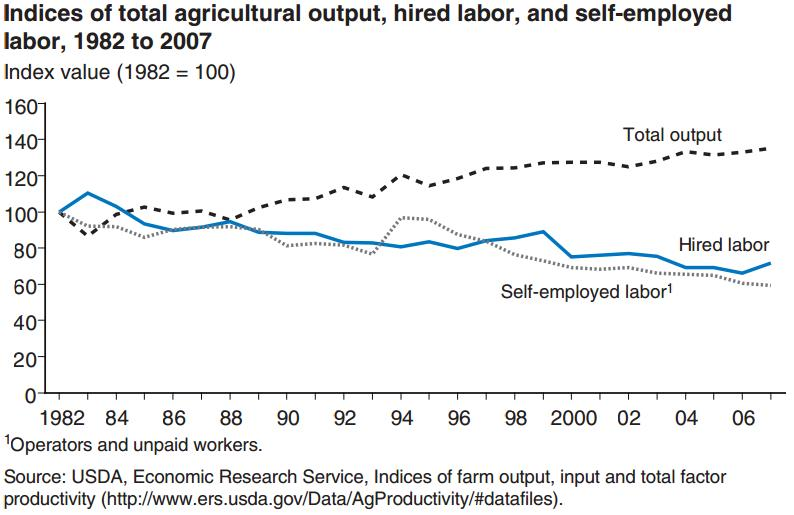
\includegraphics[scale = 0.7]{laborandoutput.jpg}
		\caption{The change labor and output in agriculture}
	\end{center}
\end{table}
Furthermore, the usage of farm machinery not only lower the amount of labor, but also increase the productivity. In late of last century, Pierre Robert proposed, developed, and popularized precision agriculture. \cite{mcbratney2005future} Under his contribution, most of the farm machinery now has the GPS, which stands for Global Positioning System, on board. With the guidance of GPS, it is very easy to plant all corps in nicely columns.  The GPS mounted farm machinery did a great job in the past few years, however, the accuracy of GPS is about $\pm$ 10 $cm$. \cite{thuilot2002automatic} This $\pm$ 10 $cm$ accuracy is acceptable with most popular 76.2 $cm$ row spacing, but not for 50.8 $cm$ or 38.1 $cm$ row spacings that will be used in the future. \cite{fawcett2014farm} And there is a place has a even higher requirement, the experiment field. The objective of the experiment field is to find the high quality breed of crops. Therefore, it is extremely important to keep the growth environment of every plant at the same level. Otherwise the experiment is meaningless. So the position to seed the experiment field is strict, every plant should has the same distance to each other. This is the precondition to provide every plant the same amount of water, sunlight, fertilizer, and carbon dioxide. So it is very necessary to have an outdoor AGV working with as high accuracy as the indoor ones.


\subsection{Knowledge gap}
For thousands of years, farming is one of the most important method to harvest food. It is a big leap from the traditional farming, which farmer could only get help from cattle or horses, to the modern farming, which farmer could get help from farm machinery. Because of the developing of farming technology, it is possible to satisfy the food demand of explosive growth of world human population. From the current situation in the United States, the products of modern farming is not only able to full fill the food demand of the United States, but also have a huge surplus. For example, more than 70 percent of the volume of U.S. production of Cotton and Tree nuts were exported from 2011 to 2013 (Table 2). And the overall average annual export share of U.S. agricultural production is 20 percent since 2000. \cite{Exports}
\begin{table}[ht!]
	\begin{center}
		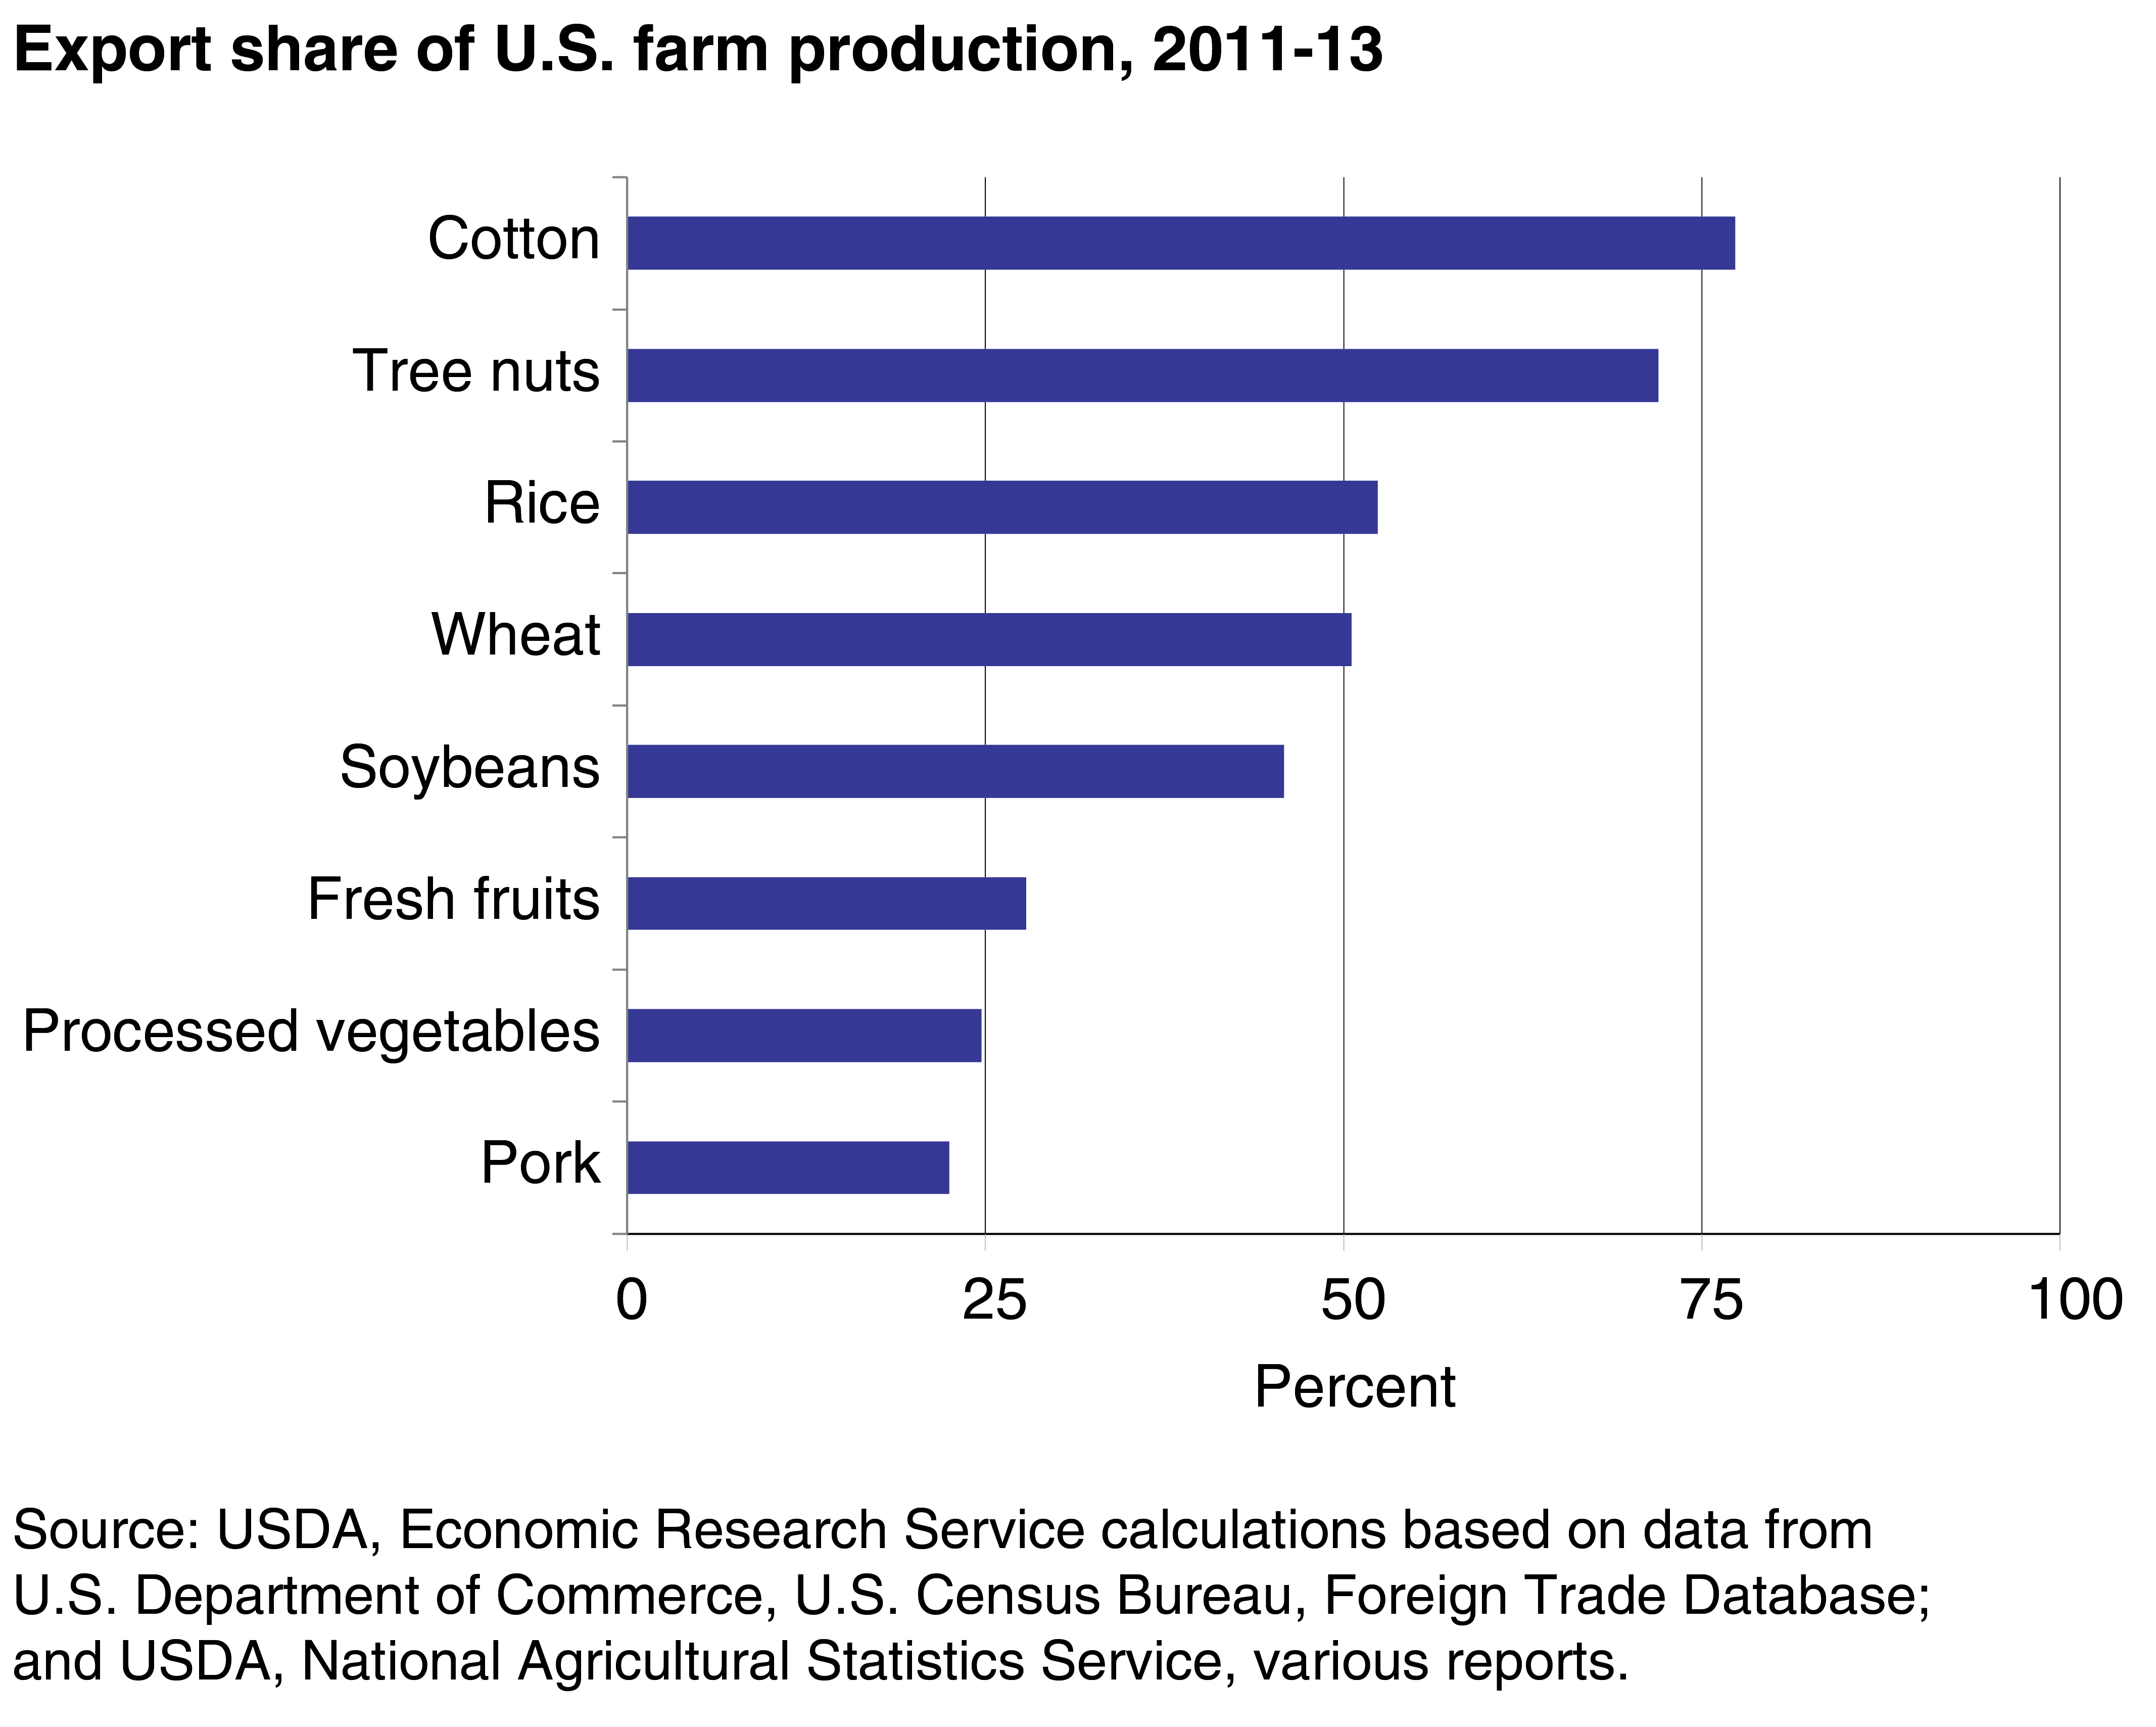
\includegraphics[scale = 0.4]{cropexport.png}
		\caption{Export share of U.S. farm production, 2011-13}
	\end{center}
\end{table}
So there is no food shortages in the U.S., and the technology of farm machinery seems to be more than enough. However, there are many places that is very hard to grow crops, because the farming conditions are totally different compare to the north America. For example, the water scarcity in West Asia and North Africa is a well-known problem. The world average annual per capita renewable supplies of water was about $7000 m^{3}$ in 1999, however, it was below $1500 m^{3}$ in West Asia and North Africa countries at the same time. More seriously, this level was $3500 m^{3}$ in 1960 and it was expected to continuously decrease to less $700 m^{3}$ by the year of 2025. \cite{margat1999water} One of a good solution for the water scarcity is to use the micro-irrigation, to be more specifically, drip irrigation (Figure 1). 
\begin{figure}[ht!]
	\begin{center}
		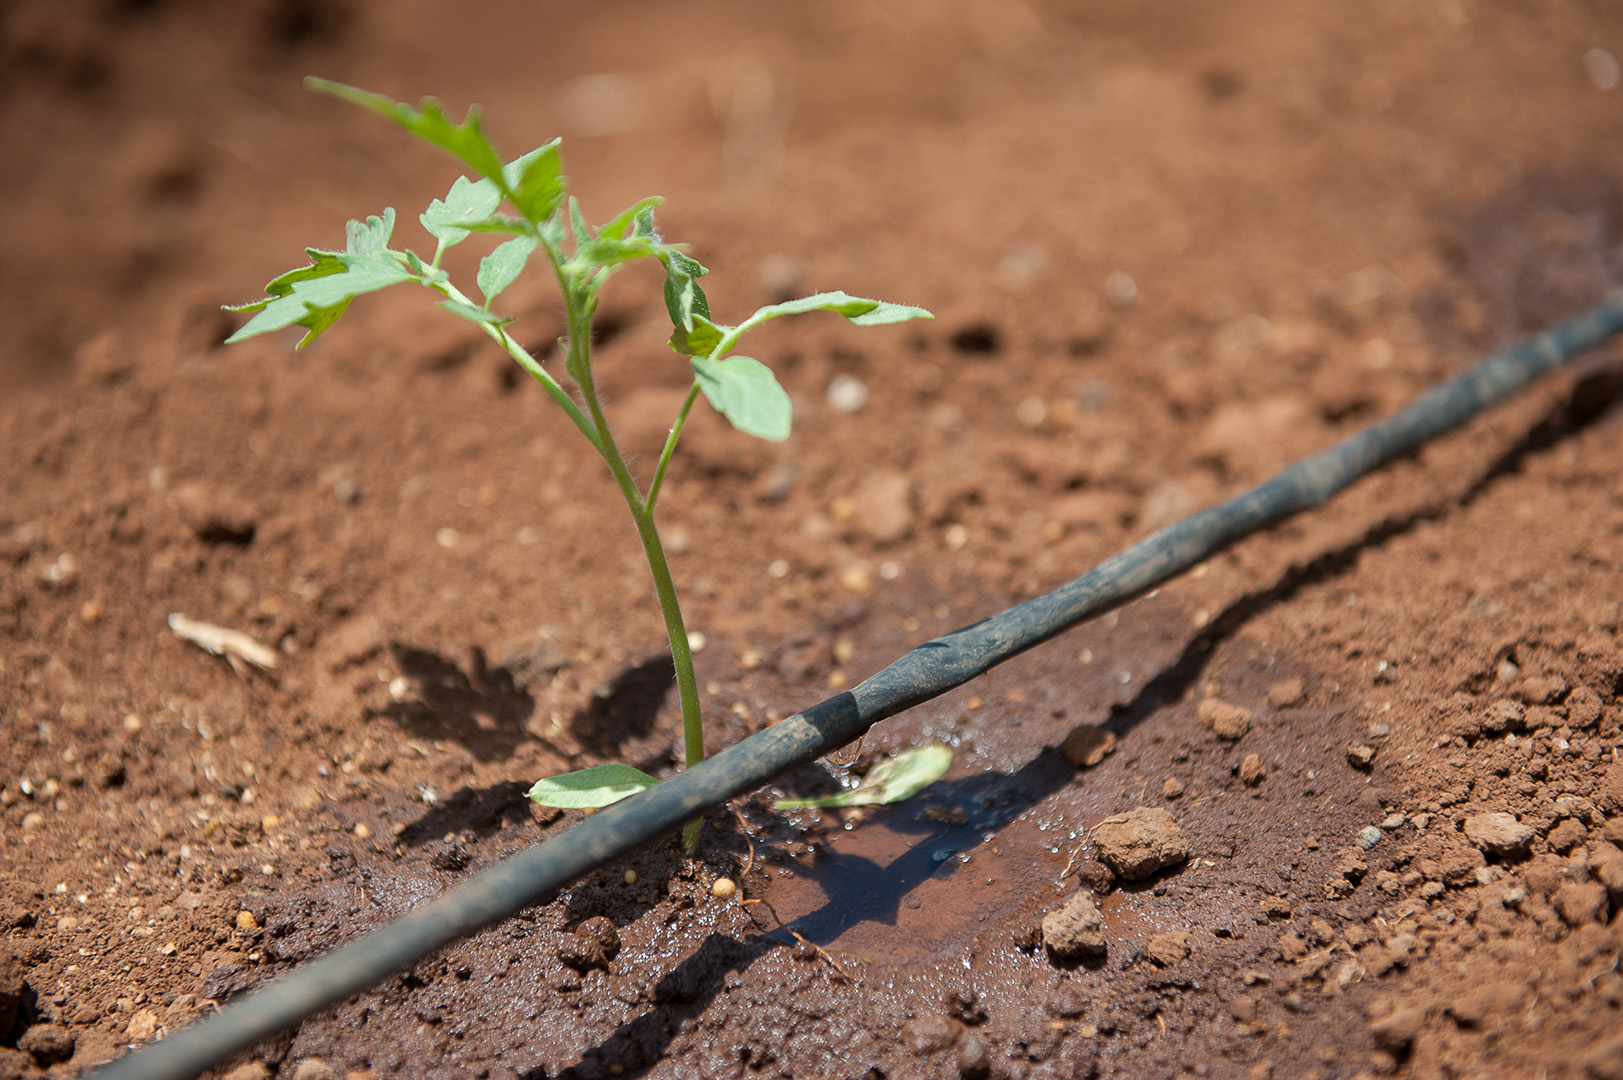
\includegraphics[scale = 0.25]{drip.jpg}
		\caption{Drip Irrigation}
	\end{center}
\end{figure}
Some advantages of micro-irrigation include improved water and nutrient management, potential for improved yields and crop quality, greater control on applied water resulting in less water and nutrient loss through deep percolation, and reduced total water requirements. \cite{phene1986advantages} However, the applications of micro-irrigation is limited. Most of micro-irrigation has been used on permanent plantings such as trees and vines. One of the reason that not using them on the field crops is because it need to be install and remove at the beginning and the end of each growing season. And a more important reason is most of the field corps are not like trees and vines, their height is low, in another word, the working zone is close to the ground. Therefore, the drip tubes make the other fields operations to become difficult than it used to be. A improved method to make it possible to use the micro-irrigation on the field corps is to bury the tubes underground. \cite{camp1998subsurface} Although the tubes neither affect the field operations nor need to be reinstalled every growing season, the position of drip spot is fixed once it was buried. So the problem turns into planting crops in the right position, which can be solved by the outdoor AGV that this paper introduced. 


\section{Background}

\subsection{Current AGVs}
The most popular guidance systems applied on current indoor AGVs are wire-guided, Optical, inertial, infrared, laser, and teaching type. \cite{KESH}
\begin{itemize}
	\item Wire-Guided:
	\begin{itemize}
		\item An energized wire is rooted along the guide path. 
		\item The antenna of the AGV follows the rooted wire.
	\end{itemize}
	The outdoor crop field is very large compare to the indoor factories. It is too expensive to root wire under ground in advance. And because of the variety of the temperature and humidity, the wire is easy to be eroded.
	\item Optical:
	\begin{itemize}
		\item Colorless florescent particles are painted on the concrete/tiled floor. 
		\item Photosensors are used to track these particles.
	\end{itemize}
	It is impossible to paint the colorless florescent particles on the soil.
	\item Inertial:
	\begin{itemize}
		\item The guide path is programmed on a microprocessor which is fixed on the AGV. 
		\item Sonar system is incorporated for finding obstacles.
	\end{itemize}
	Sonar system cannot be used as a guidance system in an open area.
	\item Infrared:
	\begin{itemize}
		\item Infrared light transmitters are used to detect the position of the vehicle.
		\item Reflectors are affixed on the top of vehicle to reflect the light.
	\end{itemize}
	It is hard to detect the position of the vehicle by using infrared light transmitters in under sunlight.
	\item Laser:
	\begin{itemize}
		\item Laser beam is used to scan wall-mounted bar-coded reflectors.
		\item Accurate positioning can be obtained.
	\end{itemize}
	This is using for a very close distance to enhance accuracy.
	\item Teaching type:
	\begin{itemize}
		\item AGV learns the guide path by moving the required route.
		\item Sends the information to the host computer.
	\end{itemize}
	The outdoor ground is rough and unpredictable. It is hard to stay in the planned route by just memorizing it. Because small errors of moving on rough ground cumulates to big errors. 
\end{itemize}
It is obvious that none of the indoor AGVs guidance systems are suitable for outdoor AGVs.

\subsection{Related researches}
\subsubsection{Sound guidance}
The sound guided vehicle was implemented with one buzzer ,which mounted on the vehicle ,and three sound receivers. Just like human can detect the position of sound source by using two ears, there was a algorithm designed with the same principle to detect the position of the buzzer. (Figure 2) 
\begin{figure}[ht!]
	\begin{center}
		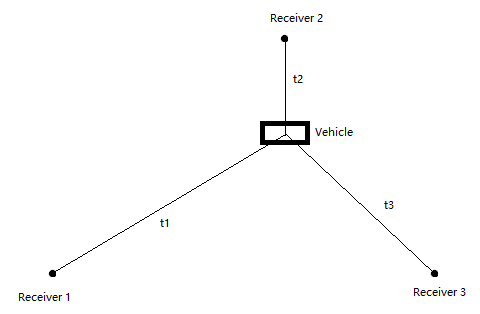
\includegraphics[scale = 1]{soundguided.png}
		\caption{Sound Guidance System}
	\end{center}
\end{figure}

On the vehicle side, the buzzer keeps emanating a cyclical audio pulse with specific signal frequency. On the guidance system side, computer recognizes and picks up the audio pulse from all three receivers. According to the time differences of receiving the same pulse, the developed algorithm is able to locate position of the vehicle. With knowledge of the vehicle location, guidance system can send the action command. The result of the experiment shows that the error is about 1 - 5 $cm$ under a velocity of 6 - 12 $cm/s$.\cite{yuping2011sound}

\subsubsection{Vision guidance}
Vision guidance is based on the information gathered by camera and dead reckoning. The developed algorithm first find a specific point in the frame, and then stare on it. From the movement of this point, the movement of vehicle is able to be reckoned. The result of the experiment shows that the error is about $5 cm$ under a velocity of $8 m/s$. However, the vehicle was tested on asphalt road. \cite{jiang2006algorithm}

\subsubsection{GPS}
GPS guidance system is one of the most reliable guidance system. There are many advantages such as low cost, portable, and able to work at any places without any pre-installation. However, the accuracy of GPS is always a problem for agriculture. An experiment in 2014 had a result that 
\begin{adjustwidth}{0.5 in}{}
	\textit{almost half (49.6\%) of all ≈68,000 GPS points recorded with the Qstarz Q1000XT GPS units fell within 2.5 m of the expected location, 78.7\% fell within 10 $m$ and the median error was 2.9 $m$. The four different types of areas showed considerable variation in the median error: 0.7 $m$ in open areas, 2.6 $m$ in half-open areas and 5.2 $m$ in urban canyons.} \cite{schipperijn2014dynamic}
\end{adjustwidth}
 
\subsubsection{Improved GPS guidance}
An improved technology for GPS, CP-DGPS (Carrier Phase Differential GPS) also named RTK GPS (Real-Time Kinematic GPS), brought the accuracy to centimeter lever. And base on the experiment had on a farm tractor, the error is lower to 10 $cm$. \cite{thuilot2002automatic} This error is acceptable with most popular 76.2 $cm$ row spacing now, but not for the 50.8 $cm$ or 38.1 $cm$ row spacing in the future. \cite{fawcett2014farm} 

\subsubsection{Sliding correction}
The ground condition of corp field is unpredictable. So the 10 $cm$ accuracy for GPS does not equivalent to 10 $cm$ accuracy for trajectory. Unlike the asphalt road, soil cannot provide constant fraction on every tires of vehicle. Sliding is a significant problem that causing trajectory error. Therefore an algorithm for sliding estimation was developed. Two inclinometers were installed to the vehicle to collect data. (Figure 3) 
\begin{figure}[ht!]
	\begin{center}
		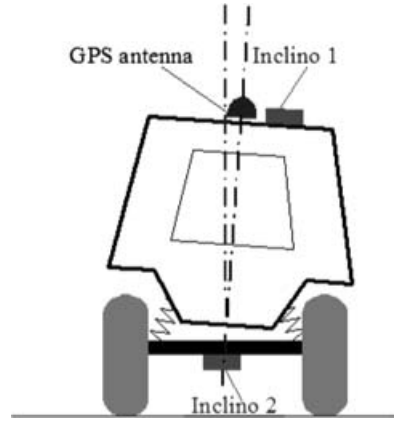
\includegraphics[scale = 0.5]{slidingcorrection.png}
		\caption{Position of inclinometers}
	\end{center}
\end{figure}
From these two tilt angles, the design algorithm can estimate the sliding and then give feedback to control system as correction. The result from this research shows that the actual trajectory error is within $\pm$ 15 $cm$. \cite{lenain2006high}

\subsection{Research question}
Based on the related researches, to achieve precision agriculture is not only to improve the accuracy of the position of farm machinery, but also to improve the accuracy of trajectory. With the localization technology, correction could be made once the vehicle off the track; with the sliding estimation technology, correction could be made once the tire slid. All the researches have done were trying to find the exact position of the vehicle or to estimate sliding then make the correction. However, to make correction means errors already occurred. To prevent error from happening, an additional device and guidance system was designed.  

\subsection{Intended project}

Driving on the farm field faces unpredictable ground conditions all the time, such as rocks, mounds, slide, rabbit or rat holes. It is impossible for tractors to drive through every thing without deviating the planned track. However, it is possible to have the attachments of the tractors always stay on the planned track. The design is to install a buffer on the tractor attachments. (Figure 4)
\begin{figure}[ht!]
	\begin{center}
		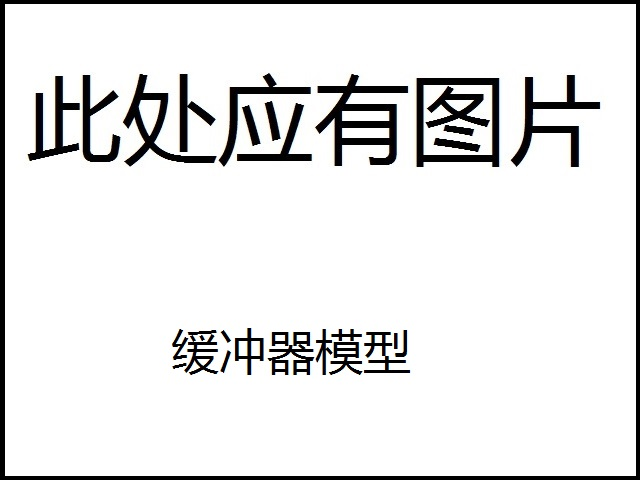
\includegraphics[scale = 0.6]{buffer.jpg}
		\caption{Buffer}
	\end{center}
\end{figure} 
The buffer allows the tractor to have some left or right displacement by providing an offset in the opposite direction to the attachment. Therefore, as long as the tractor moves in a right direction and have an accuracy that within the offset range of the buffer. The attachment is able to work in a relatively stationary condition. 

According to the related researches, vision guidance has been choose to use as the guidance system for the buffer. Because camera is a low cost device, and the imaging process algorithm is easy to be updated in the future implement. In the paper, an additional laser pointer is used as a stable reference. The laser pointer is placed at the end of rows facing to the back of tractor to provide the guidance. (Firuge 5) So that the buffer can provide the proper offset by observing the laser beam. It is expected to have a dramatically improve to the accuracy from 10 $cm$ to about 2 $cm$. 
\begin{figure}[ht!]
	\begin{center}
		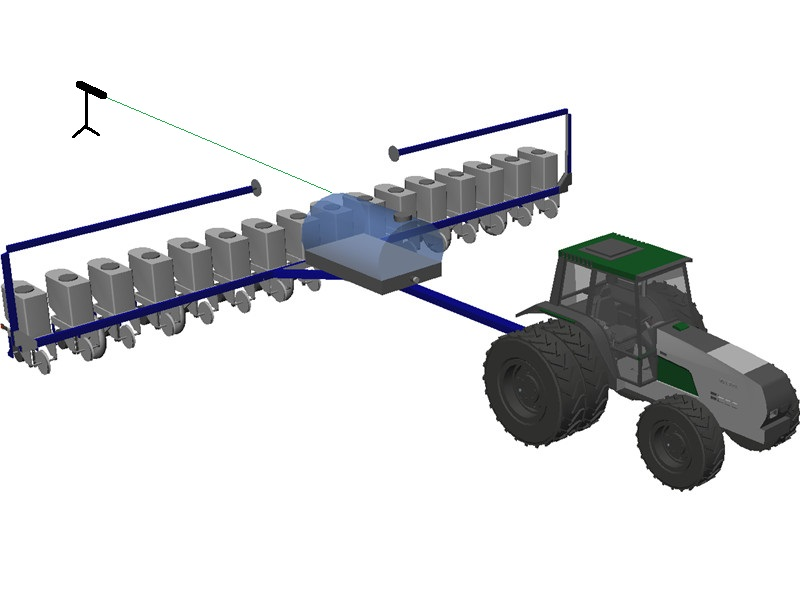
\includegraphics[scale = 0.6]{tractor.jpg}
		\caption{Laser Guidance}
		%\label{figure 1}
	\end{center}
\end{figure}



%如何能实现直线播种。借鉴室内AGV非常精准的解决方法(1),综合考虑拟人仿生.视觉(和听觉,双耳效应,引用,做图片说明)是最好的解决方案。第一步,激光引导,第二步,参照物引导,第三步,无引导,纯靠看到的图像自动选择参照物引导。激光引导分为1D 2D 3D引导。 1D左右移动,摄像头看点,2D加入前后移动,3D加入旋转,摄像头看线段。(做图片说明)

\section{Design}
The buffer is designed to be installed on the tractor attachment. And the frame of all the tools on the attachment should connect to the buffer so that they are able to move along with the buffer. At the beginning, the camera on the buffer sees the laser spot and set up the initial position. As the tractor moving, the buffer will keep maintaining the laser spot in the original position. In another word, once slide occurs on the tractor, buffer will shift the tools on the attachment to the opposite direction to prevent them from shifting. The algorithm is showing on the flow chart. (Figure 6)
% Define block styles
\tikzstyle{decision} = [diamond, draw, text width=2.5cm, text badly centered]
\tikzstyle{block} = [rectangle, draw, text width=3cm, text centered, rounded corners, minimum height=1cm]
\tikzstyle{line} = [draw, -latex']
\begin{figure}
	\begin{center}
		\begin{tikzpicture}
		\node[block](start) {Start};
		\node[block, below = 1 of start] (origin) {Initialize Position};
		\node[coordinate, below = 1cm of origin] (cycle) {};
		\node[decision, below = 2 of origin] (L) {Is left slide decteted?};
		\node[block, left = 2 of L] (goR) {Provide right offset};
		\node[decision, below = 1 of L] (R) {Is right slide decteted?};
		\node[block, left = 2 of R] (goL) {Provide left offset};
		\node[coordinate, left = 1cm of goR] (left) {};
		\node[coordinate, below = 1cm of R] (bottom) {};
		
		\path [line] (start) -- (origin);
		\path [line] (origin) -- (L);
		\path [line] (L) -- node [anchor = south] {yes} (goR);
		\path [line] (goR) -- (left) |- (cycle);
		\path [line] (L) -- node [anchor = east] {no} (R);
		\path [line] (R) -- node [anchor = south] {yes} (goL);
		\path [line] (goL) -| (left) |- (cycle);
		\path [line] (R) --  node [near start, anchor = east] {no} (bottom) -| (left) |- (cycle);
		\end{tikzpicture}
		\caption{Flow Chart}
	\end{center}
\end{figure}
\subsection{Materials and instruments}
This buffer is designed to be a implement base on current tractor attachments. In this paper, a prototype was developed for designing and experimental purpose. (Figure 6) 
\begin{figure}[ht!]
	\begin{center}
		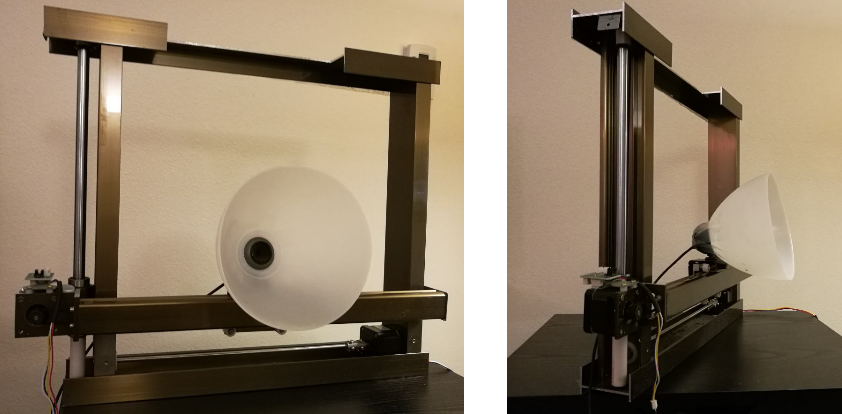
\includegraphics[scale = 0.6]{prototype.png}
		\caption{prototype}
	\end{center}
\end{figure}
A camera is installed on the top facing backwards to gather image information. A laser Pointer is placed at the end of row, facing the direction that same with the tractor moving and aiming the camera. Stepper motors are installed on the frame to provide offset for the tractor attachments. And a Raspberry Pi is used as central processor to analysis the information gathered by camera and give the action commands to stepper motors. In addition, stepper motor drivers boards are installed to transform the digital control signal to stepper motors input. The power supply was designed to use the battery of the tractor. So there is no battery in this prototype. All the parts are listed in Table 3.

\begin{table}[ht!]
	\begin{center}	
		\label{my-label}
		\begin{tabular}{|l|l|l|l|l|l|}
			\hline
			Part Name & Manufacturer & Description  & Unit Cost & Qty. & Total Cost \\ \hline
			Camera & 1 & 720P WEBCAM & 1 &1 & \\ 
			\hline
			Stepper Motor & 1 & 1 & 1 & 1 &\\ 
			\hline
			Driver boards & 1 &  1&  1&1 & \\
			\hline
			Microprocessor & 1 & Raspberry Pi 2 &  1&1 & \\
			\hline
			Frames & 1 &  1&  1&1 & \\
			\hline
			Wires & 1 &  1&  1&1 & \\
			\hline
			Camera Hood & 1 & Lampshade &  1&1 & \\
			\hline
			Curtain & 1 & Foam Board &  1&1 & \\
			\hline
			Laser Pointer & 1 & Green Laser &  1&1 & \\
			\hline
			Power Supply & 1 & Used Cellphone Charger & 1 & 3 & \\
			\hline
		\end{tabular}
		\caption{Parts List}
	\end{center}
\end{table}

%对现有农机进行改装,所以成本低。现在实验阶段使用的是,电源,树莓派,摄像头,步进马达,框架,幕布,激光。(做图表,列出成本)

\subsection{Laser guided}

Laser pointer is a low cost and efficient way to provide a straight and stable reference. Therefore, laser guidance is selected to be the guidance system. However, there is a safety problem. Laser pointer is dangerous to eyes. High power laser pointers are able to damage retina if the distance is too close. So the restriction of power of laser pointer is the lower the better.  A 5 $mW$ laser pointer is chosen, because it can be simply powered by a 3 $V$ lithium battery, and the maximum distance from which the spot on the screen can be seen is over 300 $m$ which is far enough for row of crop field. (Figure 7)
\begin{figure}[ht!]
	\begin{center}
		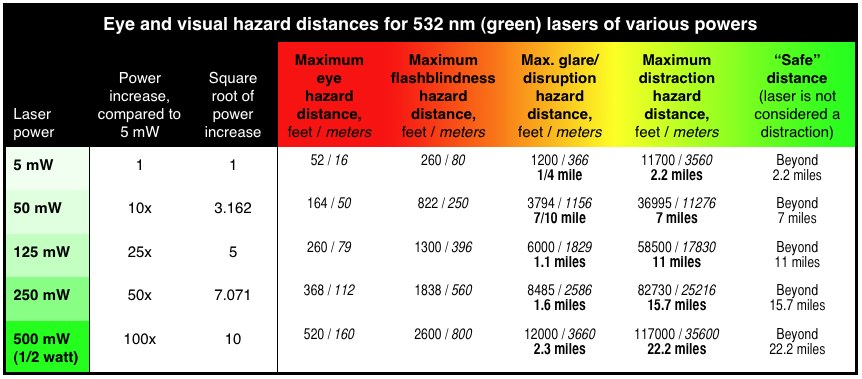
\includegraphics[scale = 0.5]{laserrange.jpg}
		\caption{Laser Range}
		%\label{figure 1}
	\end{center}
\end{figure}

\subsubsection{Imaging processing}




This is the Animal or human subject clearance. This is the Animal or human subject clearance. This is the Animal or human subject clearance. This is the Animal or human subject clearance. This is the Animal or human subject clearance. This is the Animal or human subject clearance. This is the Animal or human subject clearance. This is the Animal or human subject clearance. This is the Animal or human subject clearance. This is the Animal or human subject clearance. This is the Animal or human subject clearance. This is the Animal or human subject clearance. 
\begin{figure}[ht!]
	\begin{center}
		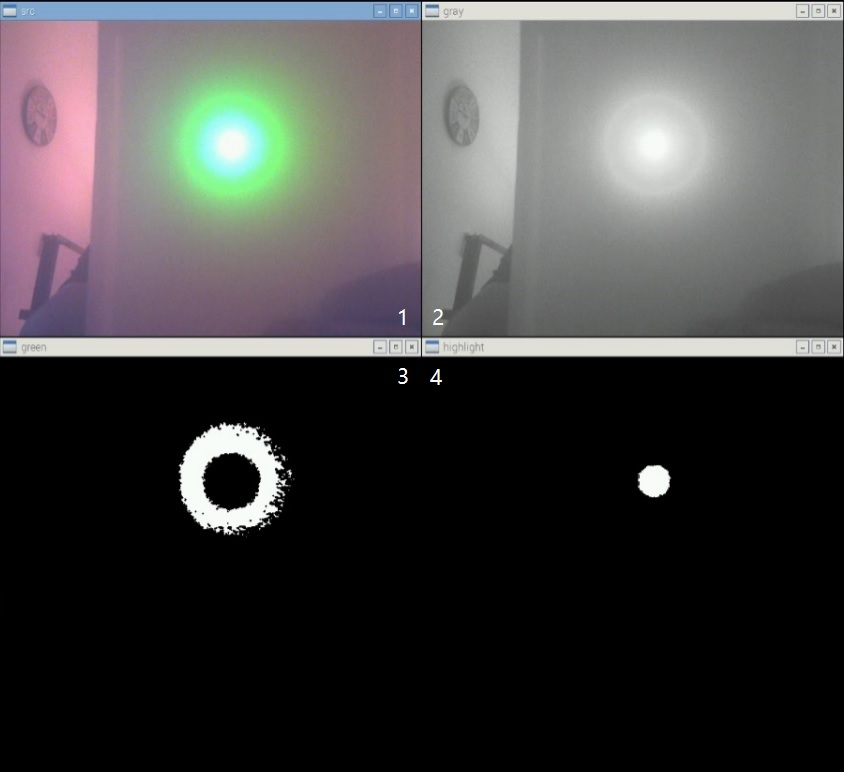
\includegraphics[scale = 0.6]{imaging.jpg}
		\caption{Imaging}
		%\label{figure 1}
	\end{center}
\end{figure}
This is the Animal or human subject clearance. This is the Animal or human subject clearance. This is the Animal or human subject clearance. This is the Animal or human subject clearance. This is the Animal or human subject clearance. This is the Animal or human subject clearance. This is the Animal or human subject clearance. This is the Animal or human subject clearance. This is the Animal or human subject clearance. This is the Animal or human subject clearance. This is the Animal or human subject clearance. This is the Animal or human subject clearance. This is the Animal or human subject clearance. This is the Animal or human subject clearance. 
用摄像头采集幕布上的光斑( 做图片,截图),分析其位置( 算法和公式),做出反馈。 给农机信号,使其左右转弯来保持直线轨迹。同时给缓冲器信号,使播种设备保持位置。

\subsubsection{Buffer design}
This is the buffer design. This is the buffer design. This is the buffer design. This is the buffer design. This is the buffer design. This is the buffer design. This is the buffer design. This is the buffer design. This is the buffer design. 
\begin{figure}[ht!]
	\begin{center}
		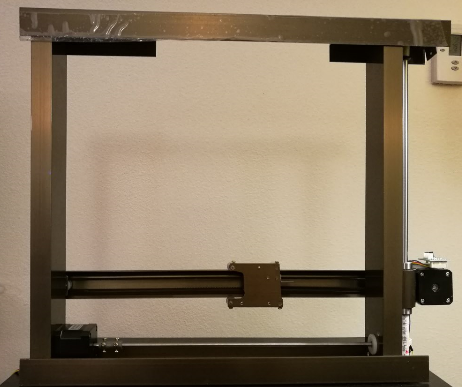
\includegraphics[scale = 0.8]{fram.png}
		\caption{Frame}
		%\label{figure 1}
	\end{center}
\end{figure}
This is the buffer design. This is the buffer design. This is the buffer design. This is the buffer design. This is the buffer design. This is the buffer design. This is the buffer design. This is the buffer design. This is the buffer design. 
\begin{figure}[ht!]
	\begin{center}
		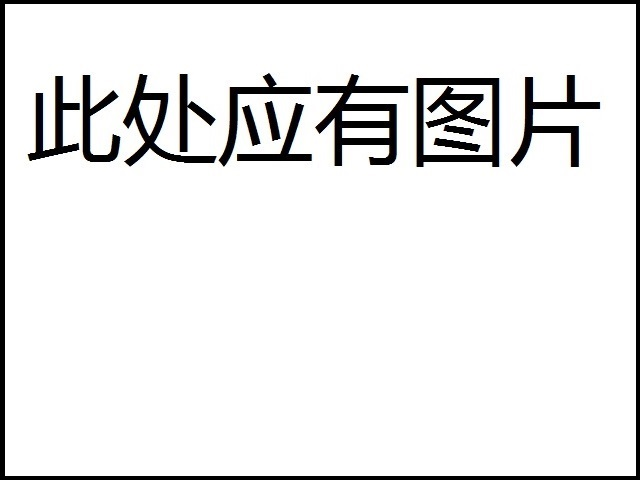
\includegraphics[scale = 0.6]{2D.jpg}
		\caption{2D}
		%\label{figure 1}
	\end{center}
\end{figure}
This is the buffer design. This is the buffer design. This is the buffer design. This is the buffer design. This is the buffer design. This is the buffer design. This is the buffer design. This is the buffer design. This is the buffer design. This is the buffer design. 
步进马达接收信号,在轨道上带着摄像头和播种设备移动。(做图片)首先实现1D移动,(做图片)再实现2D移动。

\subsubsection{Improvement}
This is the improvement. This is the improvement. This is the improvement. This is the improvement. This is the improvement. This is the improvement. This is the improvement. This is the improvement. This is the improvement. This is the improvement. 
\begin{figure}[ht!]
	\begin{center}
		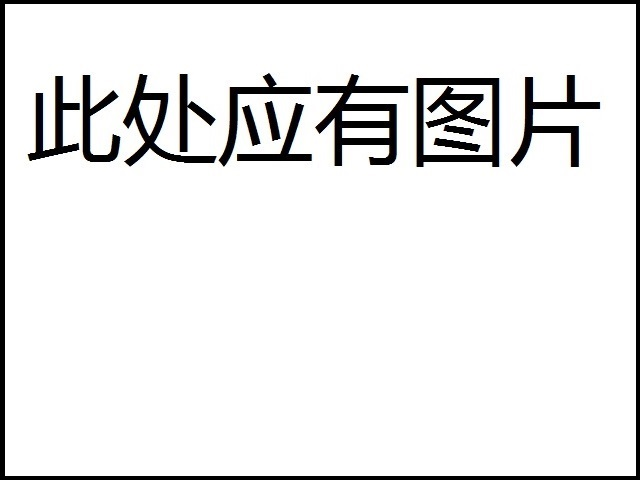
\includegraphics[scale = 0.6]{3D.jpg}
		\caption{3D}
		%\label{figure 1}
	\end{center}
\end{figure}
This is the improvement. This is the improvement. This is the improvement. This is the improvement. This is the improvement. This is the improvement. This is the improvement. This is the improvement. This is the improvement. This is the improvement. This is the improvement. This is the improvement. This is the improvement. 
\begin{figure}[ht!]
	\begin{center}
		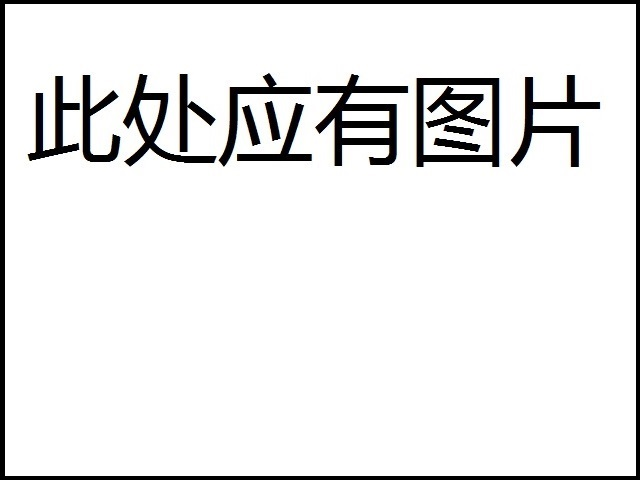
\includegraphics[scale = 0.6]{curtain.jpg}
		\caption{Curtain}
		%\label{figure 1}
	\end{center}
\end{figure}
This is the improvement. This is the improvement. This is the improvement. This is the improvement. 
为实现3D移动,摄像头需要旋转( 做图片CAD),幕布需要特制,要能显示激光的线段而不是点( 做图片CAD)。图像处理的算法和公式。

\subsection{Object guided}
This is the object guided. This is the object guided. This is the object guided. This is the object guided. This is the object guided. This is the object guided. This is the object guided. This is the object guided. This is the object guided. This is the object guided. This is the object guided. This is the object guided. This is the object guided. This is the object guided. This is the object guided. This is the object guided. This is the object guided. 
\begin{figure}[ht!]
	\begin{center}
		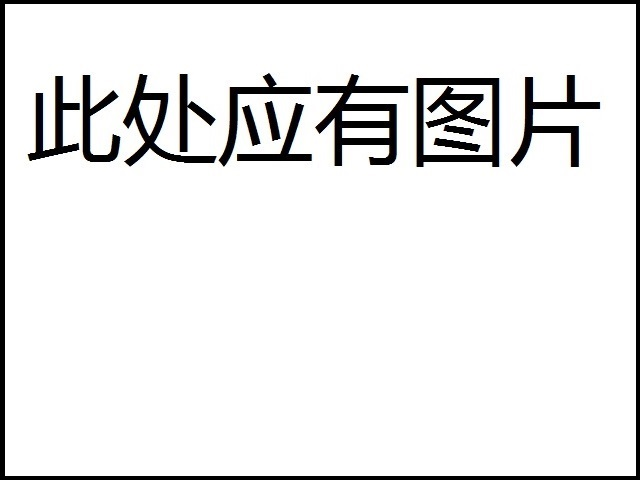
\includegraphics[scale = 0.6]{objectperspective.jpg}
		\caption{Objectperspective}
		%\label{figure 1}
	\end{center}
\end{figure}
This is the object guided. This is the object guided. This is the object guided. This is the object guided. This is the object guided. This is the object guided. This is the object guided. This is the object guided. This is the object guided. This is the object guided. 
在田边放置鲜明物体,例如交通锥Traffic Cone,通过摄像头识别该物体进行导航。少许透视算法,保持物体在屏幕中间好算,公式 ( 做图片)

\subsection{Vision guided}
This is the vision guided. This is the vision guided. This is the vision guided. This is the vision guided. This is the vision guided. This is the vision guided. This is the vision guided. This is the vision guided. This is the vision guided. This is the vision guided. This is the vision guided. This is the vision guided. This is the vision guided. This is the vision guided. This is the vision guided. This is the vision guided. This is the vision guided. This is the vision guided. This is the vision guided. This is the vision guided. This is the vision guided. This is the vision guided. This is the vision guided. This is the vision guided. This is the vision guided. This is the vision guided. This is the vision guided. This is the vision guided. This is the vision guided. This is the vision guided. This is the vision guided. This is the vision guided. This is the vision guided. 
\begin{figure}[ht!]
	\begin{center}
		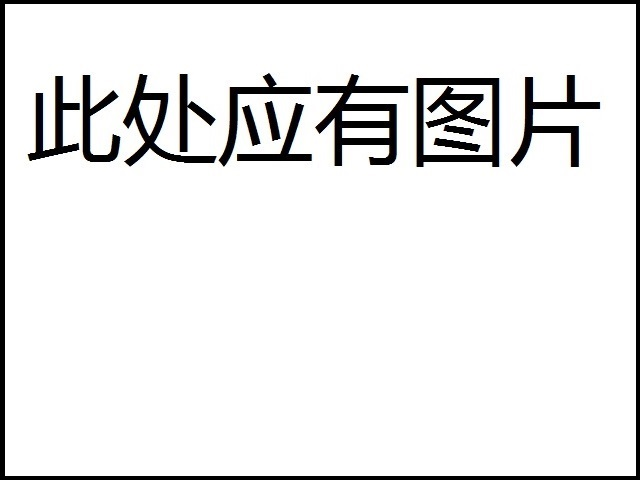
\includegraphics[scale = 0.6]{perspective.jpg}
		\caption{Perspective}
		%\label{figure 1}
	\end{center}
\end{figure}
This is the vision guided. This is the vision guided. This is the vision guided. This is the vision guided. 
不使用特殊物体,程序自动选择一个易识别物体来进行导航,例如树的树干,地平线。物体不在屏幕中间,高级透视算法,公式,(做图片)

\subsection{Alternate plans: Ultrasonic guided}
This is the Alternate plans. This is the Alternate plans. This is the Alternate plans. This is the Alternate plans. This is the Alternate plans. This is the Alternate plans. This is the Alternate plans. This is the Alternate plans. This is the Alternate plans. This is the Alternate plans. This is the Alternate plans. This is the Alternate plans. This is the Alternate plans. This is the Alternate plans. This is the Alternate plans. This is the Alternate plans. This is the Alternate plans. This is the Alternate plans. This is the Alternate plans. This is the Alternate plans. This is the Alternate plans. This is the Alternate plans. This is the Alternate plans. 
\begin{figure}[ht!]
	\begin{center}
		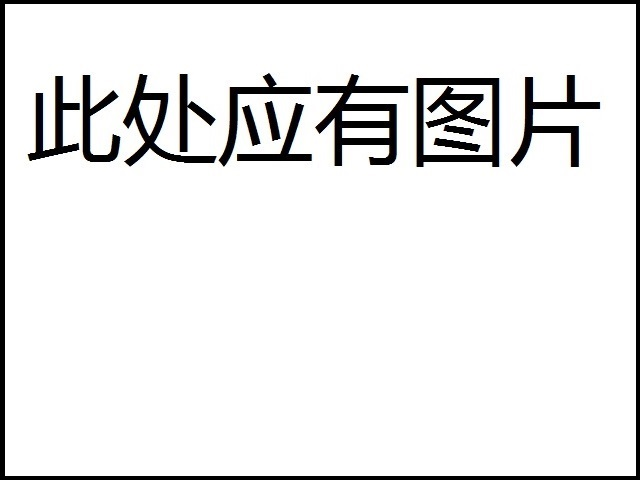
\includegraphics[scale = 0.6]{twoearsdesign.jpg}
		\caption{Twoearsdesign}
		%\label{figure 1}
	\end{center}
\end{figure}
This is the Alternate plans. This is the Alternate plans. This is the Alternate plans. This is the Alternate plans.\cite{muller1983automated} This is the Alternate plans. This is the Alternate plans. This is the Alternate plans. This is the Alternate plans. 
利用双耳效应(8引用),一个超声波源,两个接收器。生源要有特殊性,不容易被干扰,好识别。算法,公式,(做图片)

\section{Results}

\subsection{Introduction}
This is the Introduction. This is the Introduction. This is the Introduction. This is the Introduction. This is the Introduction. This is the Introduction. This is the Introduction. This is the Introduction. This is the Introduction. This is the Introduction. This is the Introduction. This is the Introduction. This is the Introduction. This is the Introduction. This is the Introduction. This is the Introduction. This is the Introduction. This is the Introduction. This is the Introduction. This is the Introduction. This is the Introduction. This is the Introduction. This is the Introduction. This is the Introduction. This is the Introduction. This is the Introduction. This is the Introduction. This is the Introduction. 
使用这个设备能达到那些效果。
,为农业育种提供方便,为未来的无人农业提供先决条件。

\subsection{Important highlights}
This is the Important highlights. This is the Important highlights. This is the Important highlights. This is the Important highlights. This is the Important highlights. This is the Important highlights. This is the Important highlights. This is the Important highlights. This is the Important highlights. This is the Important highlights. This is the Important highlights. This is the Important highlights. This is the Important highlights. This is the Important highlights. This is the Important highlights. This is the Important highlights. This is the Important highlights. This is the Important highlights. This is the Important highlights. This is the Important highlights. This is the Important highlights. This is the Important highlights. This is the Important highlights. This is the Important highlights. This is the Important highlights. This is the Important highlights. This is the Important highlights. This is the Important highlights. This is the Important highlights. 
利用摄像头来引导是趋势,摄像头成本低,易于改进,人就是靠视觉获取信息,同样机器也可以

\subsection{Feasibility}
This is the feasibility. This is the feasibility. This is the feasibility. This is the feasibility. This is the feasibility. This is the feasibility. This is the feasibility. This is the feasibility. This is the feasibility. This is the feasibility. This is the feasibility. This is the feasibility. This is the feasibility. This is the feasibility. This is the feasibility. This is the feasibility. This is the feasibility. This is the feasibility. This is the feasibility. This is the feasibility. This is the feasibility. This is the feasibility. This is the feasibility. This is the feasibility. This is the feasibility. This is the feasibility. This is the feasibility. This is the feasibility. This is the feasibility. This is the feasibility. This is the feasibility. This is the feasibility. This is the feasibility. This is the feasibility. This is the feasibility. This is the feasibility. This is the feasibility. This is the feasibility. This is the feasibility. This is the feasibility. This is the feasibility. \cite{vis2006survey}This is the feasibility. This is the feasibility. This is the feasibility. This is the feasibility. 
为实现第一步,在现有农机上进行改装,增加缓冲装置(特点),以提高精确度。制作模型进行试验。使用树莓派来对摄像头采集的图像进行处理,从而引导农机走直线。同时利用步进马达进行微调整,应付突发情况和误差。比如突然被石头搬到,突然打滑,农机突然偏离路径,无法马上回归,此时用带有步进马达的缓冲装置进行补救。而且农机很大,进行厘米级的移动困难而且耗费时间,有了缓冲装置可以减少很多误差。
现在中国的农业育种试验田非常需要。(9 引用)中国农业落后,雇佣农民成本在增加,而且他们不懂,不理解种的直的重要性。由于是在现有农机上改装,无论多落后的农机都可以。成本不高。效率高。花很少的钱能提高很多精准度。对于未来农业也很有必要。

\subsection{Constraints}
This is the constraints. This is the constraints. This is the constraints. This is the constraints. This is the constraints. This is the constraints. This is the constraints. This is the constraints. This is the constraints. This is the constraints. This is the constraints. This is the constraints. This is the constraints. This is the constraints. This is the constraints. This is the constraints. This is the constraints. This is the constraints. This is the constraints. This is the constraints. This is the constraints. This is the constraints. This is the constraints. This is the constraints. This is the constraints. This is the constraints. This is the constraints. This is the constraints. This is the constraints. This is the constraints. This is the constraints. This is the constraints. This is the constraints. This is the constraints. This is the constraints. This is the constraints. This is the constraints. \cite{vis2006survey} This is the constraints. This is the constraints. This is the constraints. This is the constraints. 
激光,物体,纯视觉,都基于摄像头,所以摄像头的限制就是这个设备的限制。图像抖动,比如光线强弱,扬尘遮挡,下雨。对于激光来说,激光的角度不太好定位,射程,功率,国标限制,不当操作对人的危害(9引用)。声音来说,声音的强度和干扰。增加声音设备,成本增加。

For the current solutions for outdoor AGV guidance system, sound guidance is not suitable for agriculture applications. Most of agricultural operation is under an open area condition. Typically the a single crop field is beyond 200 $m$ in length or width. It is difficult to recognize a sound signal with this range of distance.  High resolution microphone must be used so that it can pick up weak signal from a further distance. However, solving the long distance problem is not only just using a more expensive microphone to pick sound. The average speed of sound is 340 $m/s$ in air, and the actual speed vary along the density of air. In another word, altitude, atmospheric pressure, and humidity all can change the speed of sound. And because of the microphone is more sensitive, noise filtering is also another challenge.

坡地不好用

\subsection{Application to other areas}
This is the application to other areas. This is the application to other areas. This is the application to other areas. This is the application to other areas. This is the application to other areas. This is the application to other areas. This is the application to other areas. This is the application to other areas. This is the application to other areas. This is the application to other areas. This is the application to other areas. This is the application to other areas. This is the application to other areas. This is the application to other areas. This is the application to other areas. This is the application to other areas. This is the application to other areas. This is the application to other areas. This is the application to other areas. This is the application to other areas. This is the application to other areas. This is the application to other areas. 
不只是农业可以使用户外AGV,其他户外工作也能使用。比如修路,建筑,伐木。

\section{Conclusion}

\subsection{Importance of outdoor-AGV}
This is the importance of outdoor-AGV. This is the importance of outdoor-AGV. This is the importance of outdoor-AGV. This is the importance of outdoor-AGV. This is the importance of outdoor-AGV. This is the importance of outdoor-AGV. This is the importance of outdoor-AGV. This is the importance of outdoor-AGV. This is the importance of outdoor-AGV. This is the importance of outdoor-AGV. This is the importance of outdoor-AGV. This is the importance of outdoor-AGV. This is the importance of outdoor-AGV. This is the importance of outdoor-AGV. This is the importance of outdoor-AGV. This is the importance of outdoor-AGV. This is the importance of outdoor-AGV. This is the importance of outdoor-AGV. This is the importance of outdoor-AGV. This is the importance of outdoor-AGV. This is the importance of outdoor-AGV. This is the importance of outdoor-AGV. This is the importance of outdoor-AGV. This is the importance of outdoor-AGV. This is the importance of outdoor-AGV. This is the importance of outdoor-AGV. This is the importance of outdoor-AGV. This is the importance of outdoor-AGV. This is the importance of outdoor-AGV. This is the importance of outdoor-AGV. This is the importance of outdoor-AGV. 
本文重点讨论了关于户外AGV在农业方面的应用,现在工厂有流水线,但是室外的农业却没有这么高效率。目前来说,传统的GPS农机或许在播种上能满足现在的需求。但是要满足育种试验田的播种需求,还是需要户外AGV。放眼未来,要实现想工厂流水线一样高效的无人农业,精准的播种是第一步也是非常重要的一步。

\subsection{Overview of significants}
This is the Overview of significant findings. This is the Overview of significant findings. This is the Overview of significant findings. This is the Overview of significant findings. This is the Overview of significant findings. This is the Overview of significant findings. This is the Overview of significant findings. This is the Overview of significant findings. This is the Overview of significant findings. This is the Overview of significant findings. This is the Overview of significant findings. This is the Overview of significant findings. This is the Overview of significant findings. This is the Overview of significant findings. This is the Overview of significant findings. This is the Overview of significant findings. This is the Overview of significant findings. This is the Overview of significant findings. This is the Overview of significant findings. This is the Overview of significant findings. 
本文讨论了多种播种机器人的实现方式。使用激光简单易行,1D 2D 3D,使用物体更方便,不需要校准激光,使用视觉是最终目的,最终实现完全无人
精准度提高,因为改装,所以容易实现,实现成本低

\subsection{Limitations}
This is the limitations. This is the limitations. This is the limitations. This is the limitations. This is the limitations. This is the limitations. This is the limitations. This is the limitations. This is the limitations. This is the limitations. This is the limitations. This is the limitations. This is the limitations. This is the limitations. This is the limitations. This is the limitations. This is the limitations. This is the limitations. This is the limitations. This is the limitations. This is the limitations. This is the limitations. This is the limitations. This is the limitations. This is the limitations. This is the limitations. This is the limitations. This is the limitations. This is the limitations. This is the limitations. This is the limitations. This is the limitations. This is the limitations. This is the limitations. This is the limitations. This is the limitations. This is the limitations. This is the limitations. This is the limitations. This is the limitations. This is the limitations. 
美国农业粗放,地多,资源多,不需要这么精打细算。但是世界上的其他地区还是需要的,无人机的精准农业能带来可观的效益。虽然现在技术上不完善,但无人农业是大趋势。这个户外AGV也可以应用的很多其他的领域。

\subsection{Further improvement}
This is the Recommendations for further research. This is the Recommendations for further research. This is the Recommendations for further research. This is the Recommendations for further research. This is the Recommendations for further research. This is the Recommendations for further research. This is the Recommendations for further research. This is the Recommendations for further research. This is the Recommendations for further research. This is the Recommendations for further research. This is the Recommendations for further research. This is the Recommendations for further research. This is the Recommendations for further research. This is the Recommendations for further research. This is the Recommendations for further research. This is the Recommendations for further research. This is the Recommendations for further research. This is the Recommendations for further research. This is the Recommendations for further research. \cite{wu2004modeling}
圆形轨迹,适应不同地形,如山地,梯田。不只是播种,可以浇水施肥撒药,采摘水果,看颜色,熟的摘。实现无人农业。



\newpage
\section{REFERENCES}
\bibliographystyle{apalike}
\bibliography{bibfile}

\newpage
\appendix
\renewcommand{\appendixname}{Appendix~\Alph{section}}

\section{Appendix A}
This is appendix A
% 电路图

\end{flushleft}
\end{document}
